\documentclass[aspectratio=169]{beamer}

\usetheme{Madrid}
\usecolortheme{default}
\setbeamertemplate{navigation symbols}{}
\setbeamertemplate{headline}{}
\setbeamertemplate{footline}{%
  \leavevmode%
  \hbox to \paperwidth{\hfill\usebeamerfont{page number in head/foot}\insertframenumber\hspace{1em}}%
  \vskip2pt%
}

\title{Team F: Flight Search Component}
\subtitle{Assignment \#5 - Primary Slides (Integrated Cluster Flow)}
\author{Team F}
\date{April 2026}

\begin{document}

\begin{frame}
  \titlepage
\end{frame}

\begin{frame}[plain]
  \centering
  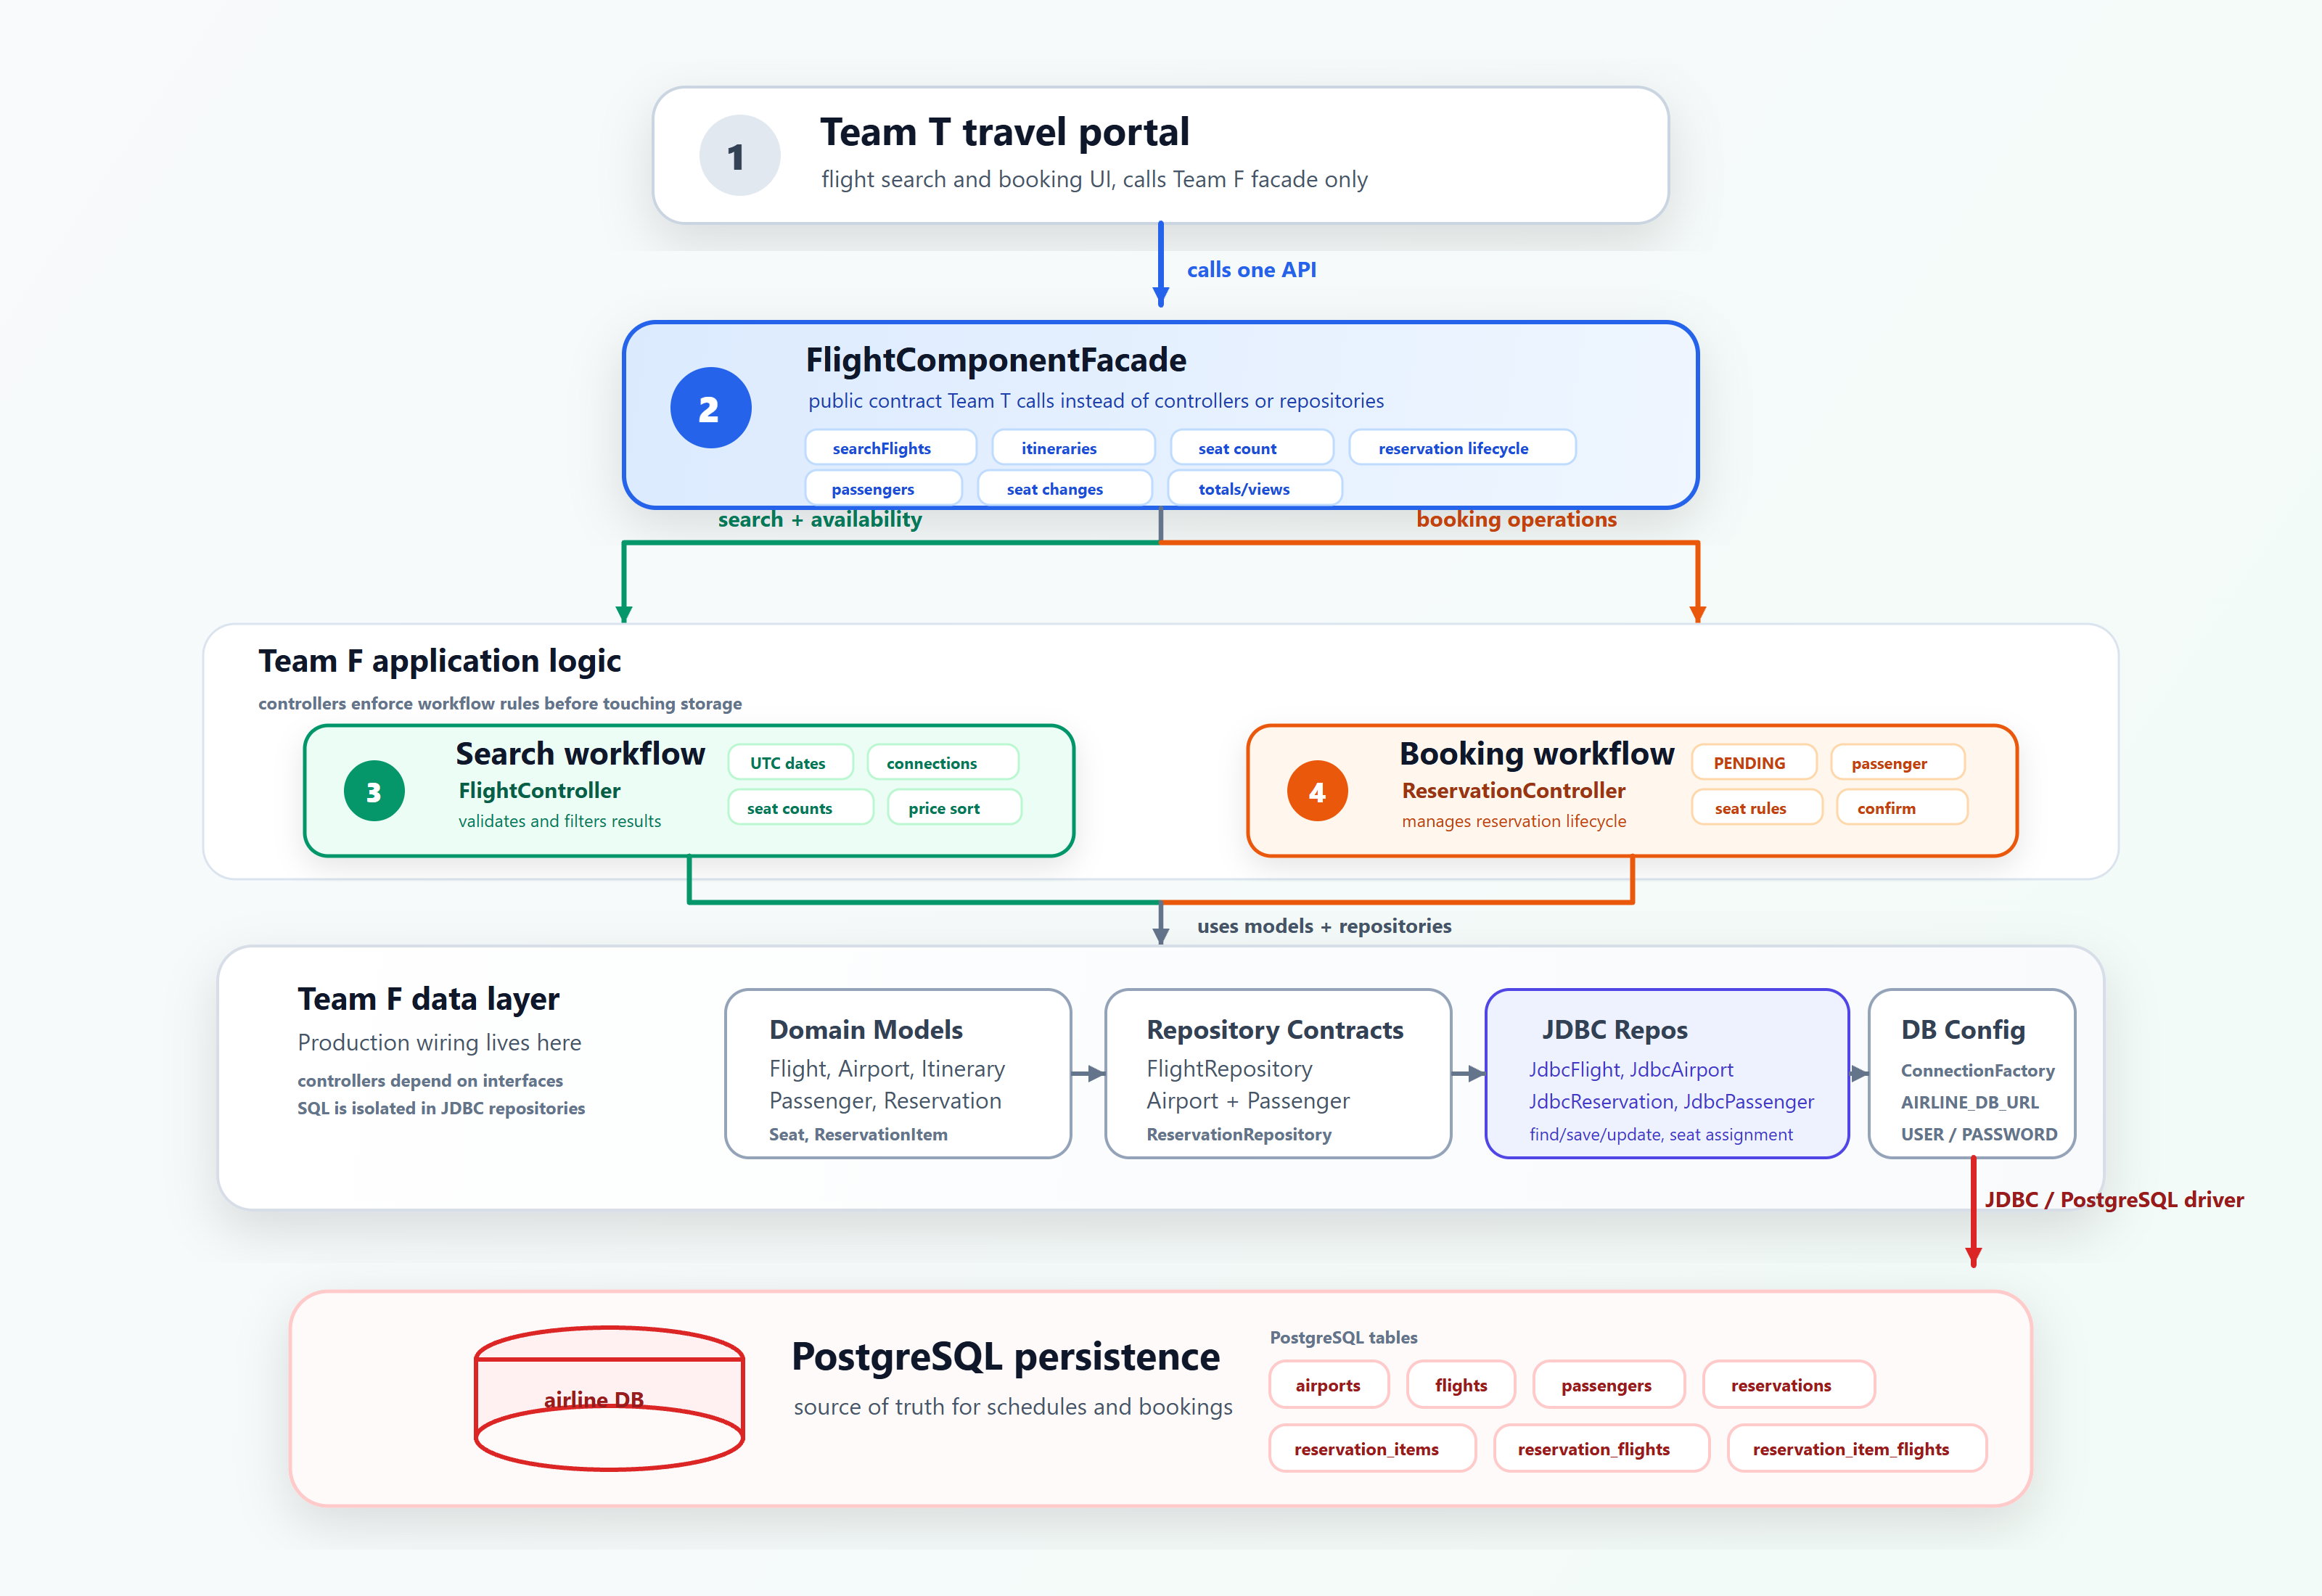
\includegraphics[width=\paperwidth,height=\paperheight,keepaspectratio]{architecture/team_f_presentation_architecture.png}
\end{frame}

\begin{frame}[plain]
  \centering
  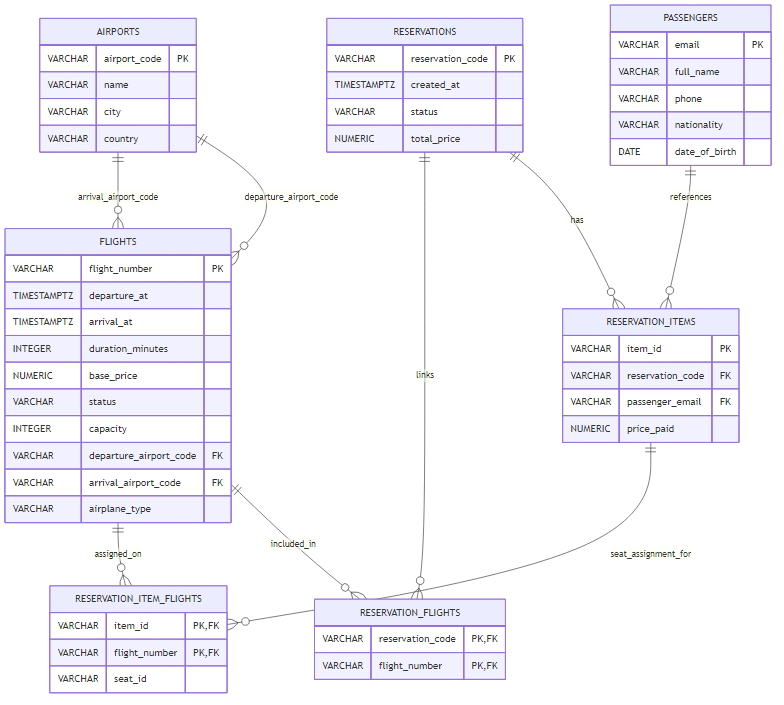
\includegraphics[width=\paperwidth,height=\paperheight,keepaspectratio]{architecture/team_f_database_erd.png}
\end{frame}

\begin{frame}{Team F Retrospective}
  \textbf{What worked}
  \begin{itemize}
    \item Internal Team F collaboration was mostly solid.
    \item Backend responsibilities became clear early.
    \item Facade contract gave a stable integration surface.
  \end{itemize}

  \vspace{0.5em}
  \textbf{Challenges}
  \begin{itemize}
    \item Some weeks had low responsiveness, which slowed decisions.
    \item Cluster-level communication with Team T was weaker than needed for smooth integration.
    \item We often had to initiate follow-up and alignment.
  \end{itemize}

  \vspace{0.5em}
  \textbf{Lessons learned}
  \begin{itemize}
    \item Define fixed cross-team check-ins early.
    \item Assign a clear integration owner per team.
    \item Lock integration milestones earlier in the semester.
  \end{itemize}
\end{frame}

\end{document}
